\section{Method}
\label{sec:method}
Our approach, in line with previous methods, builds upon a pre-trained VLM, CLIP \cite{clip}. In this section, we detail the construction of our MMRL framework and the implementation specifics.

\subsection{Preliminary}
We begin by defining the notations used in our approach. CLIP comprises two encoders: an image encoder $\mathcal{V}$ and a text encoder $\mathcal{W}$.

\noindent \textbf{Image Encoding:} The image encoder $\mathcal{V}$ consists of $L$ transformer \cite{transformer} layers, denoted $\{\mathcal{V}_i\}_{i=1}^{L}$. Given an input image \( x \in \mathbb{R}^{H \times W \times 3} \), it is divided into \( M \) fixed-size patches, each projected into a patch embedding, resulting in \( E_0 \in \mathbb{R}^{M \times d_v} \), where $M$ represents the number of patches and $d_v$ the embedding dimension. The initial patch embeddings $E_0$ are combined with a learnable class token $c_0$ and positional encodings, forming the input sequence for the transformer layers. Each layer processes this sequence as
\begin{equation}
    [c_i, E_i] = \mathcal{V}_i([c_{i-1}, E_{i-1}]) \quad
    i = 1, 2, \ldots, L
    \nonumber
\end{equation}
After passing through all transformer layers, a patch projection layer, $P_v^c$, projects the output of the class token, $c_L$, into a shared V-L latent space,
\begin{equation}
    f = P_v^c(c_L)
    \nonumber
\end{equation}
where $f \in \mathbb{R}^{d}$.

\noindent \textbf{Text Encoding:} For an input text, \eg, ``A photo of a [CLASS].", it is tokenized and converted into embeddings $T_0 \in \mathbb{R}^{N \times d_t}$, where $N$ is the token length and $d_t$ the embedding dimension. Beginning-of-text (BOT) and end-of-text (EOT) tokens, denoted $b_0$ and $e_0$, mark the sequence boundaries. These token embeddings, with positional encodings, are passed through the text encoder's $L$ transformer layers, $\{\mathcal{W}_i\}_{i=1}^{L}$, as follows,
\begin{equation} 
    [b_i, T_i, e_i] = \mathcal{W}_i([b_{i-1}, T_{i-1}, e_{i-1}]) \quad i = 1, \ldots, L 
    \nonumber
\end{equation} 
After the final layer, the output of the EOT token, $e_L$, is projected into the shared V-L space using $P_t$,
\begin{equation} 
    w = P_{t}(e_{L}) \nonumber
\end{equation} 
where $w \in \mathbb{R}^{d}$.

\noindent \textbf{Classification with CLIP:} With the image feature $f$ and text features $\{w_c\}_{c=1}^C$ for $C$ classes, CLIP calculates the cosine similarity between $f$ and each $w_c$,
\begin{equation} 
    \text{sim}(f, w_c) = \frac{f \cdot w_c}{|f| |w_c|}, \nonumber 
\end{equation} 
where $|\cdot|$ represents the $L_2$ norm. Class probabilities are then computed using the softmax function,
\begin{equation} 
    p(y = c \mid f) = \frac{\exp(\text{sim}(f, w_c) / \tau)}{\sum_{i=1}^{C} \exp(\text{sim}(f, w_i) / \tau)} \nonumber 
\end{equation} 
where $\tau$ is a temperature parameter. The final predicted class is selected as the one with the highest probability score.

% The predicted class $\hat{y}$ is determined by: \begin{equation} 
%     \hat{y} = \arg\max_{c} , p(y = c \mid f). \nonumber
% \end{equation}


%-------------------------------------------------------------------------
\begin{figure*}[tb]
\setlength{\abovecaptionskip}{0.2cm}   %调整图片标题与图距离
\setlength{\belowcaptionskip}{-0.4cm}   %调整图片标题与下文距离
\centering
\setlength{\belowcaptionskip}{-0.39cm}   %调整图片标题与下文距离
  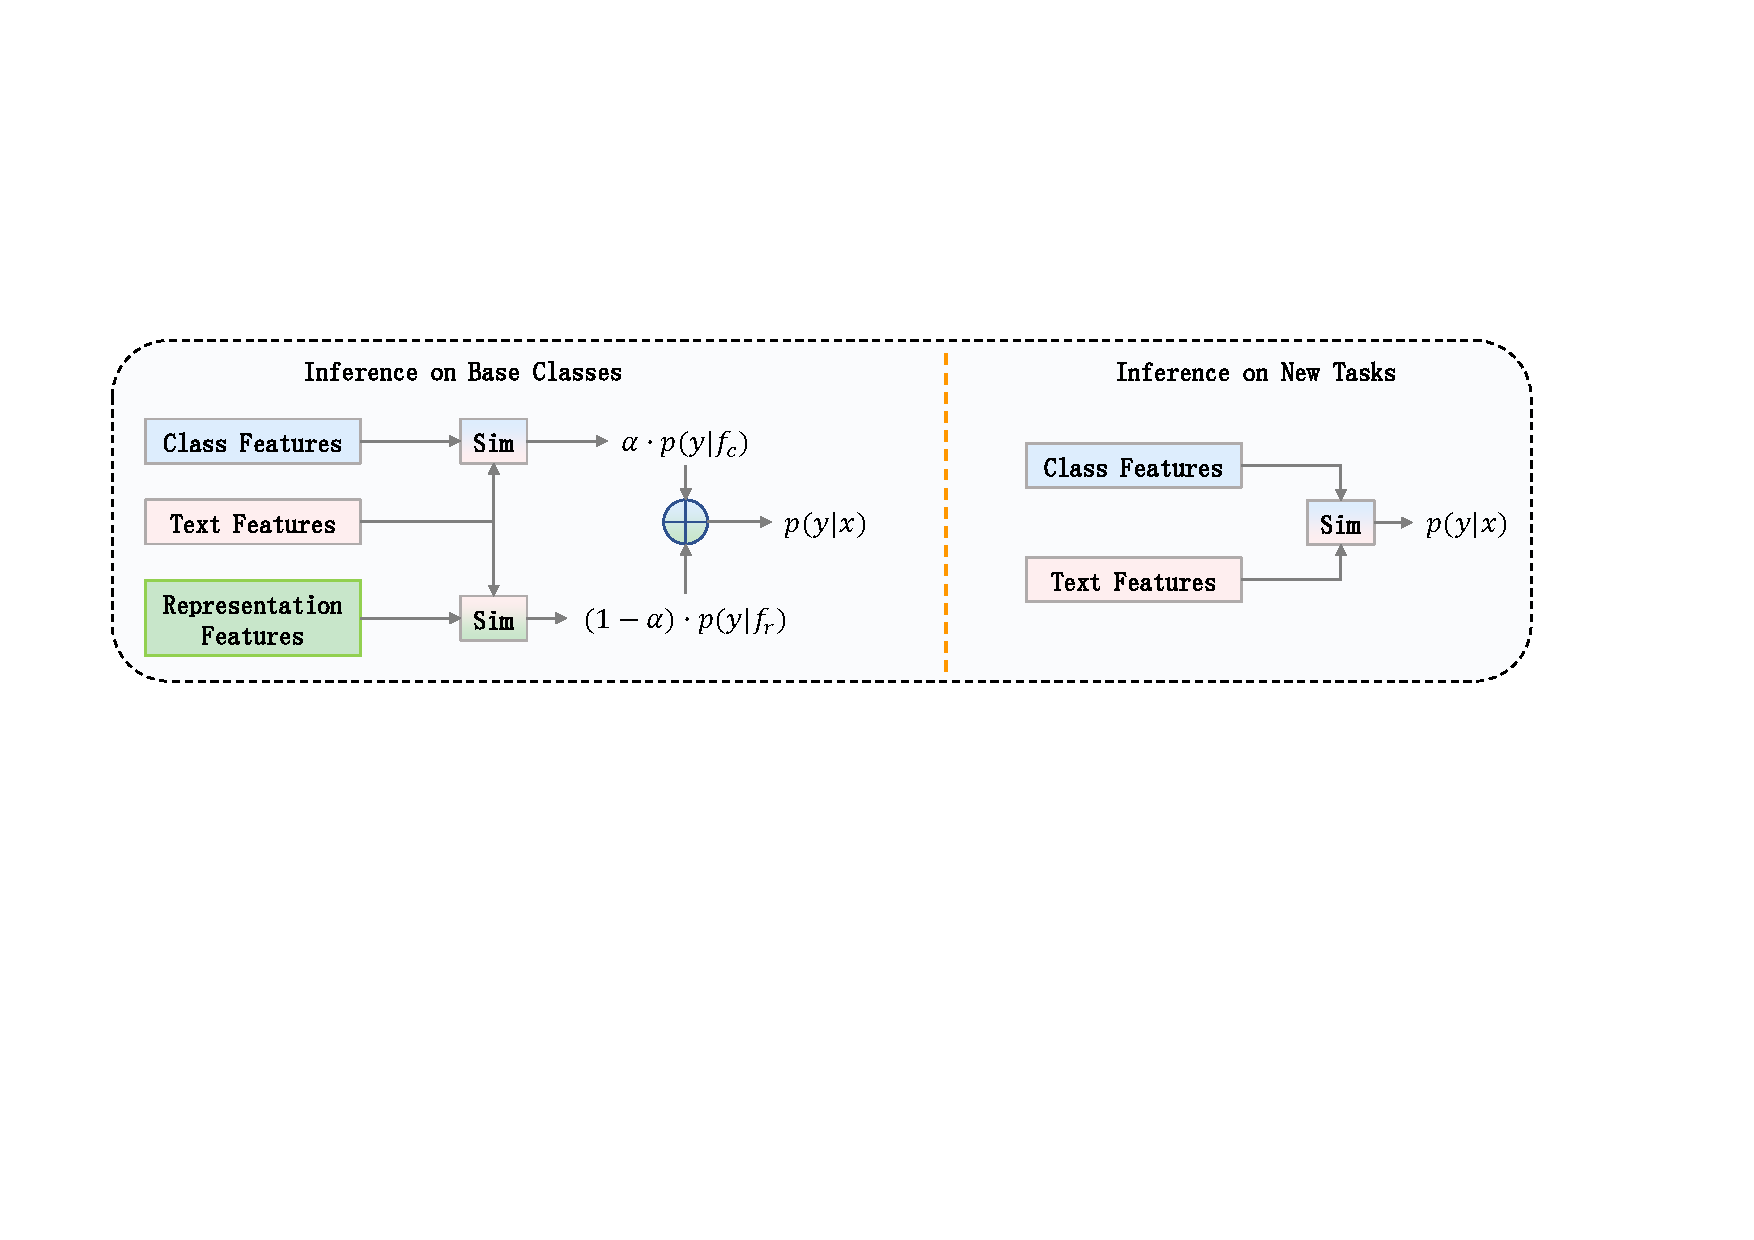
\includegraphics[width=0.7\linewidth]{fig/frame2.pdf}
  \caption{MMRL inference process, where different tasks utilize distinct features.}
  \label{framework2}
\end{figure*}
%-------------------------------------------------------------------------


\subsection{Multi-Modal Representation Learning (MMRL)} Our proposed MMRL aims to address the challenges of adapting pre-trained VLMs using few-shot data while maintaining generalization to new tasks. The training and inference frameworks of MMRL are shown in \cref{framework1} and \cref{framework2}, respectively. In the following, we describe the specifics of the methodology.


\subsubsection{Learnable Representation Space}
MMRL establishes a shared, learnable representation space $\mathcal{R}$ to facilitate multimodal interactions, initialized through sampling from a Gaussian distribution. Using a learnable mapping function $\mathcal{F}(\cdot)$, implemented as a linear layer, we project the tokens $R \in \mathbb{R}^{K \times d_r}$ in this space—where $K$ is the number of tokens and $d_r$ is the dimension of the representation space—into both visual and textual modalities,
\begin{align}
    R^v = \{R_i^v\}_{i=J-1}^{L-1} \quad & R_i^v = \mathcal{F}_i^v(R) \nonumber \\ 
    R^t = \{R_i^t\}_{i=J-1}^{L-1} \quad & R_i^t = \mathcal{F}_i^t(R) \nonumber 
\end{align}
where $R_i^v \in \mathbb{R}^{K \times d_v}$ and $R_i^t \in \mathbb{R}^{K \times d_t}$ represent the representation tokens for visual and textual modalities, respectively, in the $(i+1)$-th transformer layer. The index $J$ indicates the starting layer from which these representation tokens are integrated into the encoders.


\subsubsection{Integration into Higher Encoder Layers}
To preserve the generalized knowledge in the lower layers of the pre-trained CLIP model, the representation tokens $\mathcal{R}^v$ and $\mathcal{R}^t$ are integrated into the higher layers of the image encoder $\mathcal{V}$ and the text encoder $\mathcal{W}$, beginning from the $J$-th layer.


For the image encoder $\mathcal{V}$,
\begin{align}
    [c_i, E_i] &= \mathcal{V}_i([c_{i-1}, E_{i-1}]) \quad i = 1, \ldots, J-1 \nonumber \\  
    [c_i, \_, E_i] &= \mathcal{V}_i([c_{i-1}, R_{i-1}^v, E_{i-1}]) \quad i = J, \ldots, L - 1 \nonumber \\
    [c_i, R_i^v, E_i] &= \mathcal{V}_i([c_{i-1}, R_{i-1}^v, E_{i-1}]) \quad i = L \nonumber
\end{align}

For the text encoder $\mathcal{W}$, while previous prompt learning \cite{maple} involves replacing parts of $T_i$ to incorporate deep prompts, we retain the entire $T_i$ and insert $R_i^t$ before it, aiming to preserve the original textual information,
\begin{align}
    [b_i, T_i, e_i] &= \mathcal{W}_i([b_{i-1}, T_{i-1}, e_{i-1}]) \quad i = 1, \ldots, J-1 \nonumber \\  
    [b_i, \_, T_i, e_i] &= \mathcal{W}_i([b_{i-1}, R_{i-1}^t, T_{i-1}, e_{i-1}]) \nonumber \\
    &\hspace{4cm} i = J, \ldots, L-1 \nonumber \\
    [b_i, R_i^t, T_i, e_i] &= \mathcal{W}_i([b_{i-1}, R_{i-1}^t, T_{i-1}, e_{i-1}]) \quad i = L \nonumber
\end{align}
Note that due to the autoregressive nature of the text encoder, we adjust the attention mask matrix to accommodate the increased embedding length.


\subsubsection{Representation Learning}
Representation learning is designed to leverage representation tokens for dataset-specific adaptation, while the class token preserves the pre-trained knowledge of the original CLIP. Through a set of strategies aimed at retaining generalization during both training and inference, MMRL enables flexible inference for different tasks, as detailed below.


\begin{itemize} 

\item \textbf{Training Phase:} We optimize the features of both the representation tokens and the original class token, with the primary focus on representation features to preserve pre-trained knowledge. Specifically, the projection layer for the representation tokens is trainable, while that for the class token remains fixed. For the image encoder $\mathcal{V}$, after passing through $L$ transformer layers, we obtain the output $c_L \in \mathbb{R}^{d_v}$ for the class token and $R_L^v \in \mathbb{R}^{K \times d_v}$ for the $K$ representation tokens. The final output of the representation tokens, $r_L$, is derived by averaging across the $K$ tokens,
\begin{equation}
    r_L = \text{Mean}(R_L^v) \nonumber
\end{equation}
where $r_L \in \mathbb{R}^{d_v}$. We then apply the patch projection layers to map the outputs of both the class and representation tokens into the common V-L latent space, yielding the class features $f_c$ and representation features $f_r$.
\begin{equation}
    f_c = P_v^c(c_L) \quad f_r = P_v^r(r_L) \nonumber
\end{equation}
Here, $P_v^c$ is the original, frozen patch projection layer of CLIP for class features, while $P_v^r$ for representation features is trainable.

For the text encoder $\mathcal{W}$, following the sequential nature of text, we map the EOT token $e_L$—as in the original CLIP model—after processing through $L$ transformer layers into the common V-L space, yielding the text features.
\begin{equation} 
    w = P_{t}(e_{L}) \nonumber
\end{equation}
With the image features $f_c$, $f_r$, and the text classifiers $\{w_c\}_{c=1}^C$ for $C$ classes, we apply cross-entropy loss to separately optimize the class and representation features,
\begin{align}
\setlength\abovedisplayskip{3pt}
\setlength\belowdisplayskip{3pt}
    \mathcal{L}_{ce}^c &= -\sum_c^C y_c \log p(y = c \mid f_c) \nonumber \\
    \mathcal{L}_{ce}^r &= -\sum_c^C y_c \log p(y = c \mid f_r) \nonumber
\end{align}
where $y_c = 1$ if the image $x$ belongs to class $c$, and $y_c = 0$ otherwise. To further preserve the generalization of class features, we maximize the cosine similarity between $(f_c, w)$ and the frozen CLIP features $(f_0, w_0)$, explicitly guiding the training trajectory,
\begin{equation}
    \mathcal{L}_{cos}^v = 1 - \frac{f_c \cdot f_0}{|f_c| |f_0|} \quad \mathcal{L}_{cos}^t = 1 - \frac{1}{C}\sum_c^C \frac{w^c \cdot w_0^c}{|w^c| |w_0^c|}, \nonumber
\end{equation}
The final MMRL loss function is
\begin{equation}
    \mathcal{L}_{MMRL} = \alpha \mathcal{L}_{ce}^c + (1 - \alpha) \mathcal{L}_{ce}^r + \lambda (\mathcal{L}_{cos}^v + \mathcal{L}_{cos}^t)  \nonumber
\end{equation}
where $\alpha$ controls the balance between the features, and $\lambda$ is the penalty coefficient.

\item \textbf{Testing on Base Classes:} 
For in-distribution classes seen during training, we combine the dataset-specific representation features with the class features that preserve generalizability. The probability of an in-distribution test sample $x$ belonging to the $c$-th class is
\begin{equation}
    p(y = c \mid x) = \alpha \cdot p(y = c \mid f_c) + (1-\alpha) \cdot p(y = c \mid f_r) \nonumber
\end{equation}
where $f_c$ and $f_r$ are features extracted from the class token and representation tokens, respectively.

\item  \textbf{Testing on Novel Classes:}
For classes unseen during training or for new datasets, we rely solely on the class tokens, which retain generalized knowledge.
\begin{equation}
    p(y = c \mid x) = p(y = c \mid f_c) \nonumber
\end{equation}
\end{itemize}



% Then the predicted class $\hat{y}$ is determined by, 
% \begin{equation} 
%     \hat{y} = \arg\max_{c} , p(y = c \mid x). \nonumber
% \end{equation}



\begin{table*}[t]
\centering
\setlength{\abovecaptionskip}{0.15cm}   %调整表格标题与表格距离
\caption{Comparison of MMRL with previous state-of-the-art methods on base-to-novel generalization across 11 datasets. Bold values indicate the best results. MMRL consistently enhances base class performance without compromising generalization.}
\label{base_to_novel}
\renewcommand\arraystretch{1.06}
\setlength{\tabcolsep}{2.87mm}{
\resizebox{0.85\textwidth}{!}{
    \begin{tabular}{@{}r|ccc|ccc|ccc|ccc@{}}
    \toprule
    \multirow{2}{*}{Method} &
      \multicolumn{3}{c|}{Average} &
      \multicolumn{3}{c|}{ImageNet} &
      \multicolumn{3}{c|}{Caltech101} &
      \multicolumn{3}{c}{OxfordPets} \\
     &
      Base &
      Novel &
      HM &
      Base &
      Novel &
      HM &
      Base &
      Novel &
      HM &
      Base &
      Novel &
      HM \\ \midrule
    $\text{CLIP}_{\text{ (ICML2021)}}$ &
      69.34 &
      74.22 &
      71.70 &
      72.43 &
      68.14 &
      70.22 &
      96.84 &
      94.00 &
      95.40 &
      91.17 &
      97.26 &
      94.12 \\
    $\text{CoOp}_{\text{ (IJCV2022)}}$ &
      82.69 &
      63.22 &
      71.66 &
      76.47 &
      67.88 &
      71.92 &
      98.00 &
      89.81 &
      93.73 &
      93.67 &
      95.29 &
      94.47 \\
    $\text{CoOpOp}_{\text{ (CVPR2022)}}$ &
      80.47 &
      71.69 &
      75.83 &
      75.98 &
      70.43 &
      73.10 &
      97.96 &
      93.81 &
      95.84 &
      95.20 &
      97.69 &
      96.43 \\
    $\text{ProDA}_{\text{ (CVPR2022)}}$ &
      81.56 &
      72.30 &
      76.65 &
      75.40 &
      70.23 &
      72.72 &
      98.27 &
      93.23 &
      95.68 &
      95.43 &
      97.83 &
      96.62 \\
    $\text{KgCoOp}_{\text{ (CVPR2023)}}$ &
      80.73 &
      73.60 &
      77.00 &
      75.83 &
      69.96 &
      72.78 &
      97.72 &
      94.39 &
      96.03 &
      94.65 &
      97.76 &
      96.18 \\
    $\text{MaPLe}_{\text{ (CVPR2023)}}$ &
      82.28 &
      75.14 &
      78.55 &
      76.66 &
      70.54 &
      73.47 &
      97.74 &
      94.36 &
      96.02 &
      95.43 &
      97.76 &
      96.58 \\
    $\text{PromptSRC}_{\text{ (ICCV2023)}}$ &
      84.26 &
      76.10 &
      79.97 &
      77.60 &
      70.73 &
      74.01 &
      98.10 &
      94.03 &
      96.02 &
      95.33 &
      97.30 &
      96.30 \\
    $\text{ProVP}_{\text{ (IJCV2024)}}$ &
      85.20 &
      73.22 &
      78.76 &
      75.82 &
      69.21 &
      72.36 &
      98.92 &
      94.21 &
      96.51 &
      95.87 &
      97.65 &
      \textbf{96.75} \\
    $\text{MetaPrompt}_{\text{ (TIP2024)}}$ &
      83.65 &
      75.48 &
      79.09 &
      77.52 &
      70.83 &
      74.02 &
      98.13 &
      94.58 &
      96.32 &
      95.53 &
      97.00 &
      96.26 \\
    $\text{TCP}_{\text{ (CVPR2024)}}$ &
      84.13 &
      75.36 &
      79.51 &
      77.27 &
      69.87 &
      73.38 &
      98.23 &
      \textbf{94.67} &
      96.42 &
      94.67 &
      97.20 &
      95.92 \\
    $\text{MMA}_{\text{ (CVPR2024)}}$ &
      83.20 &
      76.80 &
      79.87 &
      77.31 &
      71.00 &
      74.02 &
      98.40 &
      94.00 &
      96.15 &
      95.40 &
      \textbf{98.07} &
      96.72 \\ \midrule
    $\text{MMRL}_{\text{ (Ours)}}$ &
      \textbf{85.68} &
      \textbf{77.16} &
      \textbf{81.20} &
      \textbf{77.90} &
      \textbf{71.30} &
      \textbf{74.45} &
      \textbf{98.97} &
      94.50 &
      \textbf{96.68} &
      \textbf{95.90} &
      97.60 &
      96.74 \\ \midrule \midrule
    \multirow{2}{*}{Method} &
      \multicolumn{3}{c|}{StanfordCars} &
      \multicolumn{3}{c|}{Flowers102} &
      \multicolumn{3}{c|}{Food101} &
      \multicolumn{3}{c}{FGVCAircraft} \\
     &
      Base &
      Novel &
      HM &
      Base &
      Novel &
      HM &
      Base &
      Novel &
      HM &
      Base &
      Novel &
      HM \\ \midrule
    $\text{CLIP}_{\text{ (ICML2021)}}$ &
      63.37 &
      74.89 &
      68.65 &
      72.08 &
      77.80 &
      74.83 &
      90.10 &
      91.22 &
      90.66 &
      27.19 &
      36.29 &
      31.09 \\
    $\text{CoOp}_{\text{ (IJCV2022)}}$ &
      78.12 &
      60.40 &
      68.13 &
      97.60 &
      59.67 &
      74.06 &
      88.33 &
      82.26 &
      85.19 &
      40.44 &
      22.30 &
      28.75 \\
    $\text{CoOpOp}_{\text{ (CVPR2022)}}$ &
      70.49 &
      73.59 &
      72.01 &
      94.87 &
      71.75 &
      81.71 &
      90.70 &
      91.29 &
      90.99 &
      33.41 &
      23.71 &
      27.74 \\
    $\text{ProDA}_{\text{ (CVPR2022)}}$ &
      74.70 &
      71.20 &
      72.91 &
      97.70 &
      68.68 &
      80.66 &
      90.30 &
      88.57 &
      89.43 &
      36.90 &
      34.13 &
      35.46 \\
    $\text{KgCoOp}_{\text{ (CVPR2023)}}$ &
      71.76 &
      75.04 &
      73.36 &
      95.00 &
      74.73 &
      83.65 &
      90.50 &
      91.70 &
      91.09 &
      36.21 &
      33.55 &
      34.83 \\
    $\text{MaPLe}_{\text{ (CVPR2023)}}$ &
      72.94 &
      74.00 &
      73.47 &
      95.92 &
      72.46 &
      82.56 &
      90.71 &
      \textbf{92.05} &
      \textbf{91.38} &
      37.44 &
      35.61 &
      36.50 \\
    $\text{PromptSRC}_{\text{ (ICCV2023)}}$ &
      78.27 &
      74.97 &
      76.58 &
      98.07 &
      76.50 &
      85.95 &
      90.67 &
      91.53 &
      91.10 &
      42.73 &
      \textbf{37.87} &
      40.15 \\
    $\text{ProVP}_{\text{ (IJCV2024)}}$ &
      80.43 &
      67.96 &
      73.67 &
      98.42 &
      72.06 &
      83.20 &
      90.32 &
      90.91 &
      90.61 &
      \textbf{47.08} &
      29.87 &
      36.55 \\
    $\text{MetaPrompt}_{\text{ (TIP2024)}}$ &
      76.34 &
      75.01 &
      75.48 &
      97.66 &
      74.49 &
      84.52 &
      \textbf{90.74} &
      91.85 &
      91.29 &
      40.14 &
      36.51 &
      38.24 \\
    $\text{TCP}_{\text{ (CVPR2024)}}$ &
      80.80 &
      74.13 &
      77.32 &
      97.73 &
      75.57 &
      85.23 &
      90.57 &
      91.37 &
      90.97 &
      41.97 &
      34.43 &
      37.83 \\
    $\text{MMA}_{\text{ (CVPR2024)}}$ &
      78.50 &
      73.10 &
      75.70 &
      97.77 &
      75.93 &
      85.48 &
      90.13 &
      91.30 &
      90.71 &
      40.57 &
      36.33 &
      38.33 \\ \midrule
    $\text{MMRL}_{\text{ (Ours)}}$ &
      \textbf{81.30} &
      \textbf{75.07} &
      \textbf{78.06} &
      \textbf{98.97} &
      \textbf{77.27} &
      \textbf{86.78} &
      90.57 &
      91.50 &
      91.03 &
      46.30 &
      37.03 &
      \textbf{41.15} \\ \midrule \midrule
    \multirow{2}{*}{Method} &
      \multicolumn{3}{c|}{SUN397} &
      \multicolumn{3}{c|}{DTD} &
      \multicolumn{3}{c|}{EuroSAT} &
      \multicolumn{3}{c}{UCF101} \\
     &
      Base &
      Novel &
      HM &
      Base &
      Novel &
      HM &
      Base &
      Novel &
      HM &
      Base &
      Novel &
      HM \\ \midrule
    $\text{CLIP}_{\text{ (ICML2021)}}$ &
      69.36 &
      75.35 &
      72.23 &
      53.24 &
      59.90 &
      56.37 &
      56.48 &
      64.05 &
      60.03 &
      70.53 &
      77.50 &
      73.85 \\
    $\text{CoOp}_{\text{ (IJCV2022)}}$ &
      80.60 &
      65.89 &
      72.51 &
      79.44 &
      41.18 &
      54.24 &
      92.19 &
      54.74 &
      68.69 &
      84.69 &
      56.05 &
      67.46 \\
    $\text{CoOpOp}_{\text{ (CVPR2022)}}$ &
      79.74 &
      76.86 &
      78.27 &
      77.01 &
      56.00 &
      64.85 &
      87.49 &
      60.04 &
      71.21 &
      82.33 &
      73.45 &
      77.64 \\
    $\text{ProDA}_{\text{ (CVPR2022)}}$ &
      78.67 &
      76.93 &
      77.79 &
      80.67 &
      56.48 &
      66.44 &
      83.90 &
      66.00 &
      73.88 &
      85.23 &
      71.97 &
      78.04 \\
    $\text{KgCoOp}_{\text{ (CVPR2023)}}$ &
      80.29 &
      76.53 &
      78.36 &
      77.55 &
      54.99 &
      64.35 &
      85.64 &
      64.34 &
      73.48 &
      82.89 &
      76.67 &
      79.65 \\
    $\text{MaPLe}_{\text{ (CVPR2023)}}$ &
      80.82 &
      78.70 &
      79.75 &
      80.36 &
      59.18 &
      68.16 &
      94.07 &
      73.23 &
      82.35 &
      83.00 &
      78.66 &
      80.77 \\
    $\text{PromptSRC}_{\text{ (ICCV2023)}}$ &
      82.67 &
      78.47 &
      80.52 &
      83.37 &
      62.97 &
      71.75 &
      92.90 &
      73.90 &
      82.32 &
      87.10 &
      78.80 &
      82.74 \\
    $\text{ProVP}_{\text{ (IJCV2024)}}$ &
      80.67 &
      76.11 &
      78.32 &
      83.95 &
      59.06 &
      69.34 &
      \textbf{97.12} &
      72.91 &
      83.29 &
      \textbf{88.56} &
      75.55 &
      81.54 \\
    $\text{MetaPrompt}_{\text{ (TIP2024)}}$ &
      82.26 &
      79.04 &
      80.62 &
      83.10 &
      58.05 &
      68.35 &
      93.53 &
      75.21 &
      83.38 &
      85.33 &
      77.72 &
      81.35 \\
    $\text{TCP}_{\text{ (CVPR2024)}}$ &
      82.63 &
      78.20 &
      80.35 &
      82.77 &
      58.07 &
      68.25 &
      91.63 &
      74.73 &
      82.32 &
      87.13 &
      \textbf{80.77} &
      83.83 \\
    $\text{MMA}_{\text{ (CVPR2024)}}$ &
      82.27 &
      78.57 &
      80.38 &
      83.20 &
      \textbf{65.63} &
      73.38 &
      85.46 &
      \textbf{82.34} &
      83.87 &
      86.23 &
      80.03 &
      82.20 \\ \midrule
    $\text{MMRL}_{\text{ (Ours)}}$ &
      \textbf{83.20} &
      \textbf{79.30} &
      \textbf{81.20} &
      \textbf{85.67} &
      65.00 &
      \textbf{73.82} &
      95.60 &
      80.17 &
      \textbf{87.21} &
      88.10 &
      80.07 &
      \textbf{83.89} \\ \bottomrule
    \end{tabular}
            }
}
\vspace{-0.3cm}
\end{table*}




